\documentclass[11pt]{exam}
\usepackage{style/preamble}
\newcommand{\name}{Section 7: Regression with Observational Data Part I}


\begin{document}
\noindent
\fbox{%
  \begin{minipage}[t]{\linewidth}
    \class, \term \hfill
    \begin{center}
      \textbf{\Large \name}
    \end{center}
    \emph{\tanames} \hfill
  \end{minipage}
}
\begingroup\small

\section{Observational Studies}
Recall the tablet–test-score example. A raw comparison of schools with vs.without tablets is not causal: wealthier schools are more likely to adopt tablets and to have resources (tutoring, staffing) that raise scores. Thus treated schools could score higher even if tablets have an adverse effect.

Randomized experiments would solve this but may be too costly. A practical alternative is to compare within strata of a confounder. For instance, compare tablet and non-tablet schools within rich neighborhoods and within poor neighborhoods. If neighborhood wealth fully captures selection into tablets and affects scores (and there is overlap), then we can identify the causal effect.
\subsection{Assumptions in Observation Studies}
Lets recall our notation. Let $T$ be the treatment and $Y$ be the outcome of interest. Typically, we assume that $T \in \{0, 1\}$ but we do not impose the same on $Y$. We also observe pre-treatment covariates $\bX$ (age, gender, \ldots). Unless otherwise stated, we assume i.i.d. sampling, i.e.,
\[
    \{\bX_i, T_i, Y_i(0), Y_i(1)\}_{i=1}^n \iid \mathbb{P}^\ast,
\]
from an unknown super-population. Throughout this part of the course, we make the following assumptions.
\begin{assumption}[SUTVA]\label{ass:sutva}
We have 
\begin{enumerate}
    \item \emph{No interference:} $Y_i(T_1,\dots,T_n)=Y_i(T_i)$; treatments on other units do not affect unit $i$
    \item \emph{Consistency:} $Y_i = Y_i(T_i)$; the observed outcome equals the corresponding potential outcome.
\end{enumerate}
\end{assumption}

\begin{assumption}[Strong Ignorability/Unconfoundedness]\label{ass:strong_ignorability}
    We have
    \[
    \{Y(1), Y(0)\} \ind T \mid \bX.
    \]
\end{assumption}
This means that, conditional on the observed covariates $\bX$, treatment assignment is as good as random. Once can think of strong ignorability as mini randomized experiments within each $\bX = \bx$. In other words, there are no unobserved confounders that jointly affect both $T$ and $Y$. 

\begin{center}
\begin{minipage}{0.47\linewidth}
\centering
\textit{Ignorability holds}
\[
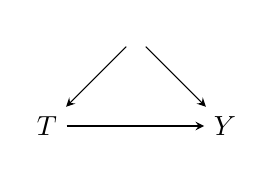
\begin{tikzpicture}[>=stealth, node distance=1.6cm]
  \node (X) {$\bX$};
  \node[below right of=X] (Y) {$Y$};
  \node[below left of=X] (T) {$T$};
  \draw[->] (X) -- (T);
  \draw[->] (X) -- (Y);
  \draw[->] (T) -- (Y);
\end{tikzpicture}
\]
No unmeasured confounding given $\bX$.
\end{minipage}\hfill
\begin{minipage}{0.47\linewidth}
\centering
\textit{Ignorability violated}
\[
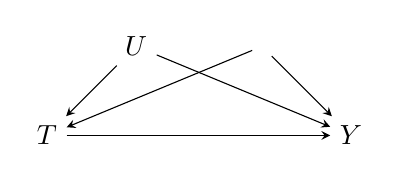
\begin{tikzpicture}[>=stealth, node distance=1.6cm]
  \node (X) {$\bX$};
  \node[left of=X] (U) {$U$};
  \node[below right of=X] (Y) {$Y$};
  \node[below left of=U] (T) {$T$};
  \draw[->] (X) -- (T);
  \draw[->] (X) -- (Y);
  \draw[->] (U) -- (T);
  \draw[->] (U) -- (Y);
  \draw[->] (T) -- (Y);
\end{tikzpicture}
\]
Unmeasured confounding given $\bX$.
\end{minipage}
\end{center}

In the tablet example, we might assume $\bX=\textit{Wealth}$ is the only confounder. If, in fact, $U=\textit{Parental Involvement}$ also influences both tablet uptake $T$ and test scores $Y$, then ignorability given $\bX$ in Assumption~\ref{ass:strong_ignorability} fails, and estimates that omit $U$ will be biased.

    \begin{center}
\begin{minipage}{0.47\linewidth}
\centering
\textit{Ignorability holds}
\[
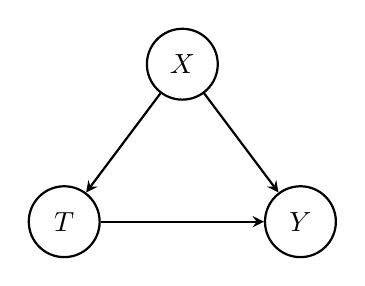
\begin{tikzpicture}[
    >=stealth,
    line width=0.8pt,
    every node/.style={circle, draw, minimum size=9mm, inner sep=0pt}
]
  % nodes
  \node (T) at (1,0)      {$T$};
  \node (Y) at (4,0)    {$Y$};
  \node (X) at (2.5, 2) {$X$};

  % edges
  \draw[->] (X) -- (Y);
  \draw[->] (X) -- (T);
  \draw[->] (T) -- (Y);
\end{tikzpicture}
\]
No unmeasured confounding given $\bX$.
\end{minipage}\hfill
\begin{minipage}{0.47\linewidth}
\centering
\textit{Ignorability violated}
\[
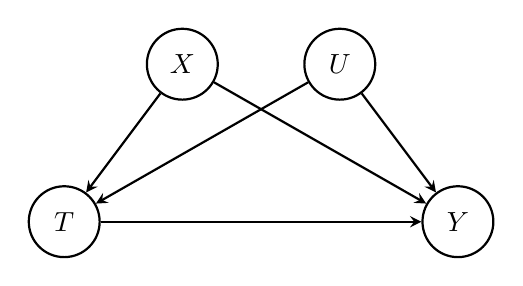
\begin{tikzpicture} [>=stealth,
    line width=0.8pt,
    every node/.style={circle, draw, minimum size=9mm, inner sep=0pt}]
  \node (T) at (1,0)      {$T$};
  \node (Y) at (6,0)    {$Y$};
  \node (X) at (2.5, 2) {$X$};
  \node (U) at (4.5, 2) {$U$};
  
  \draw[->] (X) -- (T);
  \draw[->] (X) -- (Y);
  \draw[->] (U) -- (T);
  \draw[->] (U) -- (Y);
  \draw[->] (T) -- (Y);
\end{tikzpicture}
\]
Unmeasured confounding given $\bX$.
\end{minipage}
\end{center}
\begin{itemize}
    \item If \(U\) exists and affects both \(T\) and \(Y\), then \(\{Y(1),Y(0)\} \not\!\ind T \mid X\); estimates that omit \(U\) are biased.
    \item Tablet Example: $U$ parental involvement
\end{itemize}

% \textcolor{blue}{When setting Y to Y(t) we essentially remove the arrow from T to Y and all the effects in the above DAG go through X (or (X, U)). Thus this DAG also implies Unconfoundedness this way.}

    \begin{center}
\begin{minipage}{0.47\linewidth}
\centering
\textit{Observational}
\[
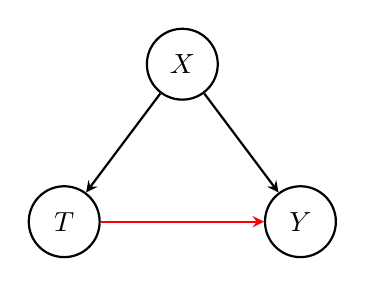
\begin{tikzpicture}[
    >=stealth,
    line width=0.8pt,
    every node/.style={circle, draw, minimum size=9mm, inner sep=0pt}
]
  % nodes
  \node (T) at (1,0)      {$T$};
  \node (Y) at (4,0)    {$Y$};
  \node (X) at (2.5, 2) {$X$};

  % edges
  \draw[->] (X) -- (Y);
  \draw[->] (X) -- (T);
  \draw[->, red] (T) -- (Y);
\end{tikzpicture}
\]
$T$ affects $Y$.
\end{minipage}\hfill
\begin{minipage}{0.47\linewidth}
\centering
\textit{Causal}
\[
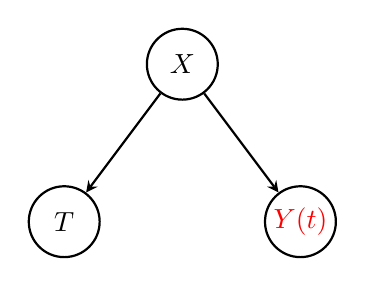
\begin{tikzpicture}[
    >=stealth,
    line width=0.8pt,
    every node/.style={circle, draw, minimum size=9mm, inner sep=0pt}
]
  % nodes
  \node (T) at (1,0)      {$T$};
  \node (Y) at (4,0)    {\textcolor{red}{$Y(t)$}};
  \node (X) at (2.5, 2) {$X$};

  % edges
  \draw[->] (X) -- (Y);
  \draw[->] (X) -- (T);
\end{tikzpicture}
\]
$T$ affects $Y(t)$ only through $\bX$.
\end{minipage}
\end{center}
\vspace{0.5em}
\begin{itemize}
    \item By setting $Y$ to level $T = t$ ($Y \to Y(t)$), we remove the arrow from $T$ to $Y$.
    \item All effects of $T$ to $Y$ go through $\bX$.  Conditioning \emph{blocks} that path.
    \item Only condition on confounder, never on collider (arrow must go into $Y$).
\end{itemize}

\begin{assumption}[Strong Overlap]\label{ass:strong_overlap}
    There exists $\eta \in (0, \frac{1}{2})$ such that
    \[
    \eta < \Pr(T = 1 \mid \bX) \leq 1 - \eta.
    \]
    \noindent 
\end{assumption}
Strong overlap ensures that for all values of $\bX$, every unit has a positive probability of receiving either treatment. Without overlap, it becomes impossible to compare treated and untreated units with similar covariates (lack of observed counterfactuals). Often, we abbreviate $e(\bx) = \Pr(T = 1\mid \bX = \bx)$, which is called the \emph{propensity score}.

In the tablet example, Assumption~\ref{ass:strong_overlap} with $\bX=\text{Wealth}$ requires that at every wealth level there are both treated and control schools. If, for instance, all wealthy schools adopt tablets, overlap fails at high $\bX$ and the causal effect there is not identified.\

\subsection{Identification and Estimation}
Given Assumptions~\ref{ass:sutva}-~\ref{ass:strong_overlap}, we can identify the $\ATE$
\begin{align*}
    \E[Y_i(1) - Y_i(0)] &= \E[\E[Y_i(1) - Y_i(0) \mid \bX_i]] \qquad \text{(Law of Iterated Expectation)}
    \\
    &= \E[\E[Y_i(1) \mid T_i = 1, \bX_i]] - \E[\E[Y_i(0)\mid T_i = 0, \bX_i]] \qquad \text{(Unconfoundedness, Overlap)}
    \\
    &= \E[\E[Y_i \mid T_i = 1, \bX_i]] - \E[\E[Y_i\mid T_i = 0, \bX_i]] \qquad \text{(SUTVA)}
    \\
    &= \E[\mu_1(\bX_i)] - \E[\mu_0(\bX_i)]
\end{align*}
where $\mu_t(\bx_i) = \E[Y_i \mid T_i = t, \bX_i = \bx_i]$. Typically, we estimate the $\ATE$ under the given assumption by first estimating $\hat \mu_t$ (e.g., via linear regression or more involved techniques) and then forming the regression estimator 
\[
    \hat \tau_{\mathrm{reg}} = \frac{1}{n} \sum_{i=1}^n \hat \mu_1(\bX_i) - \hat \mu_0(\bX_i),
\]
or the imputation estimator
\[
    \hat \tau_{\mathrm{reg-imp}} = \frac{1}{n} \sum_{i=1}^n T_i (Y_i - \hat\mu_1(\bX_i)) - (1-T_i) (\hat \mu_0(\bX_i) - Y_i).
\]

We can then either calculate the conditional or unconditional variance.
\begin{itemize}
\item \textbf{Delta method} for the conditional variance:
\[
\begin{aligned}
\Var\!\left(\hat{\tau}_{\mathrm{reg}} \mid \mathbf{X}\right)
&= \frac{1}{n^{2}}\,\Var\!\left(
\sum_{i=1}^{n} \hat{\mu}_{1}(\mathbf{X}_{i}) - \hat{\mu}_{0}(\mathbf{X}_{i})
\,\Big|\, \mathbf{X} \right) \\
&= \frac{1}{n^{2}} \Bigg[
\sum_{i=1}^{n} \big\{
\Var\!\left(\hat{\mu}_{1}(\mathbf{X}_{i}) \mid \mathbf{X}\right)
+ \Var\!\left(\hat{\mu}_{0}(\mathbf{X}_{i}) \mid \mathbf{X}\right)
- 2\,\operatorname{Cov}\!\left(\hat{\mu}_{1}(\mathbf{X}_{i}), \hat{\mu}_{0}(\mathbf{X}_{i}) \mid \mathbf{X}\right)
\big\} \\
&\hspace{2.8em}
+ \sum_{i=1}^{n}\sum_{i' \neq i}
\operatorname{Cov}\!\left(
\hat{\mu}_{1}(\mathbf{X}_{i}) - \hat{\mu}_{0}(\mathbf{X}_{i}),
\hat{\mu}_{1}(\mathbf{X}_{i'}) - \hat{\mu}_{0}(\mathbf{X}_{i'})
\mid \mathbf{X}
\right)
\Bigg].
\end{aligned}
\]
The variance expression is fairly complicated and highlights the additional dependency due to the fact that $\hat{\mu}_{t}$ is estimated from the data $\{\bX_i\}_{i=1}^n$.
\item \textbf{Bootstrap} for the unconditional variance: For $b = 1, \ldots, B$
\begin{enumerate}
\item Independently sample $n$ observations with replacement;
\item Fit a regression model and compute $\hat{\tau}^{(b)}_{\mathrm{reg}}$.
\end{enumerate}
Then calculate the sample variance of $\{\hat{\tau}^{(b)}_{\mathrm{reg}}\}_{b=1}^B$. 
\end{itemize}

\section{Sensitivity Analysis}
As we have seen above, unconfoundedness and overlap allow us to interpret association as causation. However, as we have already established previously, these assumptions are fundamentally untestable and in many applications it can be quite unlikely that these hold exactly. Sensitivity analysis examines what happens if our assumptions don't hold exactly.

\begin{quote}
    Sensitivity analysis shifts the conversation away from a binary “Do the assumptions hold?” question and to the questions like “How sensitive are my conclusions to violations of the assumptions?” or “If there were truly no causal effect,
how big would this confounding dynamic have to be to fully account for the observed effect?” It is an approach that deals in
hypotheticals to try to better understand what kinds of things could be or are unlikely to be going on. \citet[p.~59]{chazal2024causalcoursenotes}
\end{quote}

Last time, we discussed what happens when Assumption~\ref{ass:strong_overlap} of strong overlap fails. Now, we are turning to  Assumption~\ref{ass:strong_overlap} of unconfoundedness. We are going to discuss two approaches: a risk-based and a regression-based approach.

\subsection{Risk-Based Approach: Risk Ratios}
This section follows \citep{ding2016sensitivity, ding2023coursecausalinference, chazal2024causalcoursenotes}.
Assume you want to study the effect of smoking on lung cancer. \citet{doll1950smoking} reported an about nine-fold higher lung-cancer risk among smokers. \citet{fisher1957dangers} argued this association could be noncausal if an unobserved genetic factor increased both smoking and cancer risk. \citet{cornfield1959smoking} then asked: how strong must this unmeasured confounder be to explain away the observed association between cigarette smoking and lung cancer?

We replace Assumption~\ref{ass:strong_ignorability} with latent ignorability,
\[
\{Y(1),Y(0)\}\ \perp\ T \mid (\bX,U),
\]
for an unobserved confounder $U$. Thus $T$ may be confounded given $\bX$ but would be ignorable if $U$ were observed. We focus on binary $Y\in\{0,1\}$ and, binary $U\in\{0,1\}$; though the latter can be relaxed. We also omit $\bX$, but this can be generalized by conditioning all quantities on $\bX = \bx$.

Instead of the $\ATE = \E[Y(1) - Y(0)] = \Pr(Y(1) = 1) - \Pr(Y(0) = 1)$, we focus on the causal risk ratio
\[
   \RR^{\mathrm{true}}_{TY}   = \frac{\Pr(Y(1) = 1)}{\Pr(Y(0) = 1)}
\]
and test $\RR^{\text{true}}_{TY}>1$ (or $<1$). Define:
\begin{itemize}
  \item \textbf{Observed risk ratio:}\;
  $\RR^{\mathrm{obs}}_{TY}=\dfrac{\Pr(Y=1\mid T=1)}{\Pr(Y=1\mid T=0)}$ (observed effect of treatment on the outcome).
  \item \textbf{Confound--Outcome risk ratio:}\;
  $\RR_{UY}=\dfrac{\Pr(Y=1\mid U=1)}{\Pr(Y=1\mid U=0)}$ (effect of $U$ on the outcome).
  \item \textbf{Treatment--Confounder ratio:}\;
  $\RR_{TU}=\dfrac{\Pr(U=1\mid T=1)}{\Pr(U=1\mid T=0)}$ (imbalance of $U$ across treatment).
\end{itemize}
% Instead focusing on the  $\ATE = \E[Y(1) - Y(0)] = \Pr(Y(1) = 1) - \Pr(Y(0) = 1)$ and testing whether $\ATE > 0$ ($\ATE < 0$), we are considering the risk ratio 
% \[
%   \RR^{\mathrm{true}}_{TY}   = \frac{\Pr(Y(1) = 1)}{\Pr(Y(0) = 1)}
% \]
% and test whether $\RR^{\mathrm{true}}_{TY}  > 1$ ($\RR^{\mathrm{true}}_{TY} < 1$). We also define the following quantities
% \begin{itemize}
%     \item \textbf{Observed Risk Ratio}: $\RR^{\mathrm{obs}}_{TY}   = \frac{\Pr(Y = 1 \mid T = 1)}{\Pr(Y = 1 \mid T = 0)}$, the observed ratio of cancer in the smokers compared to non-smokers. 
%     \item \textbf{Risk Ratio of} $Y$ \textbf{given} $U$: $\RR_{UY}   = \frac{\Pr(Y = 1 \mid U = 1)}{\Pr(Y = 1 \mid U = 0)}$, risk of cancer in the presents of genetic factors or not
%     \item \textbf{Risk Ratio of} $U$ \textbf{given} $T$: $\RR_{TU}   = \frac{\Pr(Y = 1 \mid U = 1)}{\Pr(Y = 1 \mid U = 0)}$, prevalence of hidden factor present given smoking or not
% \end{itemize}
We can think of $\RR_{TU}$ and $\RR_{UY}$ as decomposing the causal effect of $T$ on $Y$ through the association between the unmeasured confounder $U$ and $T$ and $Y$ respectively. Hence, they are unobservable. We think about them as \emph{sensitivity} parameters. 
We then ask the question: Given we observe $\RR^{\mathrm{obs}}_{TY} > 1$ (smoking has an observed effect on lung cancer), how large must the unobserved confounding $U$ on $Y$ be (measured by $\RR_{UY}, \RR_{TY}$) to imply $\RR^{\mathrm{true}}_{TY} = 1$ (no causal effect)? If $\RR_{UY}$ or $\RR_{TY}$ are large, then this provides evidence in favor of a causal effect.

\begin{theorem}[\citet{cornfield1959smoking}, Cornfield Condition]
    Assuming $\{Y(1),Y(0)\}\ \perp\ T \mid U$. If $\RR^{\mathrm{obs}}_{TY} > 1$ then in order for $\RR^{\mathrm{true}}_{TY} = 1$ we must have 
    \[
        \min(\RR_{UY}, \RR_{TY})  \geq \RR^{\mathrm{obs}}_{TY}.
    \] 
\end{theorem}
Note that the condition $\RR^{\mathrm{obs}}_{TY} > 1$ can always be achieved by redefining $T$ as $1 - T$. However, we can even derive a more general, sharp condition.
\begin{theorem}[\citet{ding2016sensitivity}, Result~1]\label{thm:risk_sensitivity}
    Assuming $\{Y(1),Y(0)\}\ \perp\ T \mid U$. If $\RR^{\mathrm{obs}}_{TY} > 1$ then
    \[
        \RR^{\mathrm{true}}_{TY} \geq \RR^{\mathrm{obs}}_{TY} \times \frac{\RR_{TU} + \RR_{UY} - 1}{\RR_{TU} \times \RR_{UY}}.
    \]
    Further, in order for $\RR^{\mathrm{true}}_{TY} = 1$ we must have
    \[
        \max(\RR_{UY}, \RR_{TY})  \geq \RR^{\mathrm{obs}}_{TY} + \sqrt{\RR^{\mathrm{obs}}_{TY} (\RR^{\mathrm{obs}}_{TY} - 1)}.
    \]
\end{theorem}
These calculations quantify how strong unmeasured confounding must be to attenuate the observed risk ratio. Let the bias factor be
\[
\mathrm{BF}_U \;=\; \frac{\RR_{UY}\,\RR_{TU}}{\RR_{UY}+\RR_{TU}-1},
\]
which is the maximum relative amount by which unmeasured confounding can reduce $\RR^{\mathrm{obs}}_{TY}$.
\begin{example}
    If we estimate $\widehat{\RR}^{\mathrm{obs}}_{TY}=2.1$ with a 95\% CI $[1.4,\,3.1]$ and let $(\RR_{UY},\RR_{TU})=(2,2)$, then $\mathrm{BF}_U=1.33$ and
\[
\widehat{\RR}^{\mathrm{true}}_{TY}=2.1/1.33=1.58,\qquad \text{CI }[1.40/1.33,\;3.10/1.33]=[1.05,\,2.33].
\]
Such confounding cannot explain away the effect (the lower bound remains $>1$).
\end{example}

\begin{example}
    If $(\RR_{UY},\RR_{TU})=(2.5,3.5)$, then $\mathrm{BF}_U=1.75$ and
\[
\widehat{\RR}^{\mathrm{true}}_{TY}=2.1/1.75=1.20,\qquad \text{CI }[1.40/1.75,\;3.10/1.75]=[0.80,\,1.77].
\]
Here the adjusted CI includes $1$, so the association is no longer significantly $>1$.
\end{example} 

In practice, we might do:
\begin{enumerate}
  \item Compute the observed risk ratio $\widehat{\RR}^{\mathrm{obs}}_{TY}$ and its $(1-\alpha)$ CI.
  \item For a grid of $(\RR_{UY},\RR_{TU})$, plot the values for which $\widehat{\RR}^{\mathrm{true}}_{TY}$ is smaller than $1$ and also plot the values for which it is not statistically  significant.
  \item Read from the resulting curves the strength of unmeasured confounding needed to explain away the causal effect. Use domain knowledge to judge whether this is confounding is realistic.
\end{enumerate}
An illustration is given in Figure~\ref{fig:sensitivity}.


\begin{figure}
    \centering
    
\includegraphics[width=0.5\linewidth]{figures/sensitivity_plot.pdf}
    \caption{Sensitivity Plot; from \citet{ding2016sensitivity}.}
    \label{fig:sensitivity}
\end{figure}

The advantage of the risk-based approach is that it is fully non-parametric, but often only works well when the outcome is binary, $Y \in \{0, 1\}$. In contrast, the next approach discussed here relies on a parametric model, but allows $Y$ to be continuous.

\subsection{Regression-Based Approach: Omitted Variable Bias}
This section follows \citet{cinelli2020making}.
Suppose we wish to run a linear regression model of an outcome $Y$ on treatment $T$, while controlling for a sent of confounders $\bX$ (including an intercept) an $U$,
\begin{equation}\label{eq:full_model}
    Y_i = \hat \tau T_i + \hat{\bm{\beta}}^\top \bX_i + \hat{\gamma} U_i + \varepsilon_i.
\end{equation}
However, $U$ might be an unobserved confounder such that we can only run the restricted model,
\begin{equation}\label{eq:res_model}
    Y_i = \hat{\tau}_{\mathrm{res}} T_i + \hat{\bm{\beta}}_\mathrm{res}^\top \bX_i + \varepsilon_{\mathrm{res}, i}.
\end{equation}
We then ask, how does the estimated $\hat{\tau}_{\mathrm{res}}$ compare to $\hat{\tau}$? By the FWL Theorem~\ref{thm:fwl} in the Appendix, we have 
\begin{align*}
    \hat{\tau}_{\mathrm{res}} &= \frac{\sCov(T^{\perp \bX}, Y^{\perp \bX})}{\sVar(T^{\perp \bX})}
    \\
    &=  \frac{\sCov(T^{\perp \bX}, \hat \tau T^{\perp \bX} + \hat \gamma U^{\perp \bX})}{\sVar(T^{\perp \bX})}
    \\
    &= \hat \tau + \hat \gamma \frac{\sCov(T^{\perp \bX},  U^{\perp \bX})}{\sVar(T^{\perp \bX})}
    \\
    &= \hat \tau + \hat \gamma \hat \delta,
\end{align*}
where $\sVar$ and $\sCov$ are the sample variance and covariance. If the confounder $U$ in Equation~\eqref{eq:full_model} is a true confounder, then $\sCov(T^{\perp \bX},  U^{\perp \bX}) \neq 0$ and the results of the regression will be biased. The bias is given by $\widehat{\mathrm{bias}} = \hat \gamma \hat \delta$. Thus, this expression is called the \emph{omitted variable bias} (OVB) formula. 

\subsection{Interpretation and Shortcomings of the traditional Omitted Variable Bias}
The coefficient $\hat \gamma$ describes how different subgroups of confounders impact our linear predictions on the outcome. It thus captures the \emph{impact} the unobserved confounder has on the outcome.
On the other hand, $\hat \delta$ is a coefficient of the linear regression
\[
    U_i = \hat \delta T_i + \hat{\bm{\psi}}^\top \bX_i + \varepsilon_{U, i}.
\]
It described how the treatment affects the confounder when controlling for the covariates. We can think about $\hat \delta$ as a measure of \emph{imbalance} of the confounder with respect to the treatment. The OVB formula then reads: ''Impact times Imbalance".

However, \citet{cinelli2020making} point out that the traditional OVB approach is has two main disadvantages. First, it provides no sense of scale whenever $U$ is not binary. Second, it does not generalize well to multiple unnamed confounders. They propose a different approach based on the $R^2$ values (see Appendix~\ref{sec:r2} for a recap).

\subsection{$R^2$-based OVB}
\begin{theorem}[\citep{cinelli2020making}, $R^2$-based OVB]\label{thm:r2_ovb}
    Assuming Equations~\eqref{eq:full_model} and~\eqref{eq:res_model}, then the OVB can be expressed as
    \[
        |\widehat{\mathrm{bias}}| = \sqrt{\frac{R^2_{Y \sim U \mid T, \bX} R^2_{T \sim U \mid\bX}}{1 - R^2_{T \sim U \mid\bX}} \frac{\sVar(Y^{\perp T, \bX})}{\sVar(T^{\perp \bX})}}.
    \]
\end{theorem}
Theorem~\ref{thm:r2_ovb} expresses the bias in terms of the two sensitivity parameters $R^2_{Y \sim U \mid T, \bX}$ and $R^2_{T \sim U \mid\bX}$. $R^2_{Y \sim U \mid T, \bX}$ describes the variance of $Y$ explained by the confounder $U$ when controlling for $(T, \bX)$. It can capture how much variance is left to explain for an unnamed confounder, after condoning on the observed quantities. Similarly, $R^2_{T \sim U \mid\bX}$ measures the variance of $T$ attributed to $U$ when controlling for the observed covariates $\bX$.
This formulation of the OVB has multiple advantages. First, it is scale-free as $R^2 \in [0, 1]$ always. Second, it allows us to incorporate multiple unmeasured confounders. Indeed, if we would consider 
\[
    Y_i = \hat \tau T_i + \hat{\bm{\beta}}^\top \bX_i + \bm{\hat{\gamma}}^\top \bm{U}_i + \varepsilon_i.
\]
we could just define $U_i^\ast = \bm{\hat{\gamma}}^\top \bm{U}_i$ and obtain
\[
    Y_i = \hat \tau T_i + \hat{\bm{\beta}}^\top \bX_i + U_i^\ast + \varepsilon_i.
\]
Then $R^2_{Y \sim \bm{U} \mid T, \bX} = R^2_{Y \sim U^\ast \mid T, \bX}$ and $R^2_{T \sim \bm{U} \mid\bX} \leq R^2_{T \sim U^\ast \mid\bX}$. Hence the $R^2$ OVB formula for one confounder yields a conservative upper bound when considering multiple confounder.

Third, the $R^2$ formulation of the OVB allows us to conduct a variety of sensitivity analyses. Among others they derive quantities to measure how strong a unnamed confounder must be (also in relative terms to other covariates) to make a statistically significant effect not significant anymore. We can then judge whether this is sensible.

Recall the school-tablet-score example. Assume that ($R^2_{Y \sim U \mid T, X}$, $R^2_{T \sim U \mid X}$) need to be large in order to explain the the results away. Assume further that we believe that $X = \textit{Wealth}$ is the most important confounder and $(R^2_{Y \sim X \mid T}$, $R^2_{T \sim X}$) are comparably smaller than what  ($R^2_{Y \sim U \mid T, X}$, $R^2_{T \sim U \mid X}$) need to be to explain the result away. Since it is unlikely that we missed an confounder with a larger effect than wealth, it is reasonable to assume that no unmeasured confounder can overturn the result. We refer to \citet{cinelli2020making} for details.


\newpage
\section{Appendix}
We define the sample variance and covariance for two samples $\{A_i, B_i\}_{i = 1}^n$ as
\[
    \sVar(A) = \frac{1}{n - 1} \sum_{i=1}^n (A_i - \Bar{A})^2, \qquad \sCov(A, B) = \frac{1}{n-1}\sum_{i=1}^n (A_i - \Bar{A}) (B_i - \Bar{B}).
\]
where $\Bar{A} = \frac{1}{n} \sum_{i = 1}^n A_i$.

\subsection{Population Ordinary Least Squares}
Much of this section is based on \citet[Appendix~B]{ding2023coursecausalinference}. Assume $(Y_i, \bX_i) \iid \mathbb{P}$ with $Y \in \R$ and $\bX \in \R^p$. We define the population least squares coefficient as
\[
    \beta = \argmin_b \E[(Y - \bX^\top b)^2].
\]
By setting $f(b) = \E[(Y - \bX^\top b)^2]$ and differentiating, we see that any solution $\beta$ must satisfy the \emph{normal equation}
\[
    \E[\bX (Y - \bX^\top \beta)] = \bm{0}.
\]
A unique solution is obtained at
\[
    \beta = \E[\bX\bX^\top]^{-1} \E[\bX Y],
\]
whenever $\E[\bX\bX^\top]$ is invertible. Define the residual $\epsilon = Y - \bX^\top \beta$ then
\[
    \E[\bX \epsilon] = \E[\bX (Y - \bX^\top \beta)] = \E[\bX Y] - \E[\bX \bX^\top] \beta = \bm{0}.
\]

\subsubsection{Population OLS with Intercept}
If we include $1$ in $\bX$ then 
\[
    \E[\epsilon] = \E[Y - \bX^\top \beta] = 0,
\]
by the above. This further implies 
\[
    \Cov(\bX, \epsilon) = \E[\bX \epsilon] - \E[\bX] \E[\epsilon] = \bm{0}.
\]
Thus, including an intercept leads to a zero mean residual which is uncorrelated with the other variables.

\subsubsection{Univariate Population OLS with Intercept}
In the special case where $X \in \R$ we have 
\[
    (\alpha, \beta) = \argmin_{a, b} \E[(Y - a - bX)^2],
\]
with equals
\[
    \beta = \frac{\Cov(X, Y)}{\Var(X)}, \qquad \alpha = \E[Y] - \beta \E[X].
\]

\subsubsection{Univariate Population OLS without Intercept}
Without an intercept we fit
\[
    \gamma = \argmin_{\gamma} \E[(Y - \gamma X)^2],
\]
which has the explicit formula
\[
    \gamma = \frac{\E[XY]}{\E[X^2]}.
\]
Note that when $\E[X] = 0$, $\gamma = \frac{\Cov(X, Y)}{\Var(X)} = \beta$.


\subsection{Sample Ordinary Least Squares}
Consider the linear model
\[
    \bY = \bX \bm{\beta}^\ast + \bm{\varepsilon},
\]
where
  \[
  \bY =
  \begin{bmatrix}
  Y_1 \\ \vdots \\ Y_n
  \end{bmatrix}, \quad
  \bX =
  \begin{bmatrix}
  X_{11} & \cdots & X_{p1} \\
  \vdots & \ddots & \vdots \\
  X_{n1} & \cdots & X_{pn}
  \end{bmatrix}, \quad
  \bm{\beta}^\ast =
  \begin{bmatrix}
  \beta^\ast_1 \\ \vdots \\ \beta^\ast_p
  \end{bmatrix}.
\]
Since we have not specified $\bm{\varepsilon}$, this model does not impose any parametric assumption. Traditionally, estimation is done with the Ordinary Least Squares (OLS) estimator:
\[
    \hat{\bm{\beta}} = \argmin_{\bm{\beta}} \|\bY - \bX \bm{\beta}\|_2,
  \]
  which leads to the closed-form solution:
  \[
    \hat{\bm{\beta}} = (\bX^\top \bX)^{-1} \bX^\top \bY
    = \left(\frac{1}{n}\sum_{i=1}^n \bX_i \bX_i^\top\right)^{-1}
      \left(\frac{1}{n}\sum_{i=1}^n \bX_i Y_i\right),
  \]
  where $\bX_i = [X_{1i}, \ldots, X_{pi}]^\top$ and assuming that $\mathrm{rank}(\bX) = p$.
The OLS estimator gives the \emph{best linear approximation} of $\E[Y_i \mid \bX_i]$. Define the residual $\hat{\bm{\varepsilon}} = \bY - \bX \hat{\bm{\beta}}$, consider then the \emph{normal equation}
\[
    \bX^\top \hat{\bm{\varepsilon}} = \bX^\top (\bY - \bX \hat{\bm{\beta}}) = \bX^\top \bY - \bX^\top \bX \hat{\bm{\beta}} = \bm{0}.
\]
This provides another way to derive $\hat{\bm{\beta}}$, by just considering the normal equations
\[
\sum_{i = 1}^n X_{ij} \left(Y_i - \sum_{j^\prime=1}^p X_{ij^\prime} \beta_j\right) = 0 \quad \forall j = 1, \ldots, p,
\]
and solve for $\{\beta_j\}_{j=1}^p$.

% \sum_{i=1}^n \bX_i \hat{\bm{\varepsilon}}_i = \sum_{i=1}^n \bX_i (\bY_i - \bX_i^\top \hat{\bm{\beta}}) = \sum_{i=1}^n \bX_i \bY_i - \sum_{i=1}^n \bX_i^\top (\bX^\top \bX)^{-1} \bX^\top \bY
\subsubsection{Sample OLS with Intercept}
If we include $1$ in $\bX_i$ then we have 
\[
    \sum_{i=1}^n \hat{\varepsilon}_i = 0.
\]
This leads to 
\[
 \sCov(\bX_j, \hat{\bm{\varepsilon}}) = 0,
\]
where $\bX_j = [X_{1j}, \ldots, X_{nj}]^\top$.

\subsubsection{Univariate Sample OLS with Intercept}\label{sec:univeriate_sample_ols_intercept}
In the univeriate case $X_i \in \R$ where we regress
\[
    Y_i = \alpha + \beta X_i + \epsilon_i,
\]
we obtain
\[
    \hat \beta = \frac{\sCov(X, Y)}{\sVar(X)} = \frac{\sum_{i=1}^n (X_i - \Bar{X}) Y_i}{\sum_{i=1}^n (X_i - \Bar{X})^2}, \qquad \hat \alpha = \Bar{Y} - \hat \beta \Bar{X}.
\]

\subsubsection{Univariate Sample OLS without Intercept}
Without an intercept, the univeriate case $X_i \in \R$, we fit
\[
    Y_i = \gamma X_i + \epsilon_i,
\]
which has the explicit formula
\[
    \hat \gamma = \frac{\sum_{i=1}^n X_i Y_i}{\sum_{i=1}^n X_i^2} = \frac{\langle X,Y\rangle}{\|X\|^2} = \cos{(\theta_{X, Y})} \frac{\|Y\|}{\|X\|},
\]
where $\theta_{X, Y}$ is the angle between the vectors $\{X_i\}_{i=1}^n \in \R^n$ and $\{Y_i\}_{i=1}^n \R^n$.
If $\Bar{X} = 0$, then $\hat \gamma = \frac{\sCov(X, Y)}{\sVar(X)} = \hat \beta$.

\subsection{Frisch–Waugh–Lovell Theorem}
\subsubsection{Sample FWL}\label{thm:fwl}
We only discuss the sample version here. Consider the linear regression
\[
     \bY = \bX \bm{\beta} + \bZ \bm{\gamma} + \bm{\varepsilon},
\]
where $\bX \in \R^{n \times p}, \bZ \in \R^{n \times k}$. Set $\bW = [\bX, \bZ]$ then OLS provides
\[
    \begin{pmatrix}
  \hat{\bm{\beta}} \\ \hat{\bm{\gamma}} 
  \end{pmatrix} = (\bW^\top \bW)^{-1} \bW^\top \bY.
\]
In some applications however, we might only be interested in $\hat{\bm{\beta}}$ (for example if $\bX$ represents the treatment) and calculating the whole expression above can be cumbersome. Frisch–Waugh–Lovell (FWL) provide another way to obtain $\hat{\bm{\beta}}$.

In the following, for a matrix $\bA$ let 
\[
    P_{\bA} = \bA (\bA^\top \bA)^{-1} \bA^\top, \qquad M_{\bA} = I - P_{\bA},
\]
be the orthogonal projection matrix and its orthogonal compliment of the column space of $\bA$.

\begin{theorem}[Frisch–Waugh–Lovell]
Consider $\bY = \bX \bm{\beta} + \bZ \bm{\gamma} + \bm{\varepsilon}$, then to obtain $\hat{\bm{\beta}}$ we can follow these steps
\begin{enumerate}
    \item Regress $\bY \sim \bZ$ and obtain the residual $\bY^{\perp \bZ} = \bY - P_{\bZ}\bY = M_{\bZ} \bY$.
    \item Regress $\bX \sim \bZ$ (each column $\bX_j \sim \bZ$) and obtain the residual $\bX^{\perp \bZ} = \bX - P_{\bZ}\bX = M_{\bZ} \bX$.
    \item Regress $\bY^{\perp \bZ} \sim \bX^{\perp \bZ}$. Then the coefficient of that regression $\hat{\bm{\delta}} = (\bX^\top M_{\bZ} \bX)^{-1} \bX^\top M_{\bZ} \bY$ is $\hat{\bm{\beta}}$.
\end{enumerate}
\end{theorem}
Note that this is equivalent to considering the coefficient $\bm{\delta} (= \bm{\beta})$ of $\bX$ in the regression
\[
   M_{\bZ} Y = M_{\bZ} \bX \bm{\delta} + M_{\bZ} \bm{\varepsilon}.
\]
This can be immediately seen by multiplying both sides of $\bY = \bX \bm{\beta} + \bZ \bm{\gamma} + \bm{\varepsilon}$ by $M_{\bZ}$, as $M_{\bZ} \bZ = \bm{0}$.

\subsubsection{FWL in Causal Inference}
Often in causal inference we are interested in estimating the effect of an univeriate treatment $T_i$ on an univeriate outcome $Y_i \in \R$ after controlling for covariates $\bX_i \in \R^p$,
\[
    Y_i = \tau T_i + \bm{\beta}^\top \bX_i + \varepsilon_i.
\]
In this case, FWL shows its strength. Assuming that an intercept is included in $\bX_i$, then to obtain our estimate $\hat \tau$ we have the formula
\[
    \hat \tau = \frac{\sCov(T^{\perp \bX}, Y^{\perp \bX})}{\sVar(T^{\perp \bX})} = \frac{\langle T^{\perp \bX},Y^{\perp \bX}\rangle}{\|T^{\perp \bX}\|^2}.
\]
Here we recover the formula of Section~\ref{sec:univeriate_sample_ols_intercept}, where the (linear) effect of $\bX$ on the treatment and outcome is removed (partialled out). The formula holds due to $\sum_{i=1}^n T_i^{\perp \bX} = \sum_{i=1}^n Y_i^{\perp \bX} = 0$ as we include an intercept in $\bX$.

\medskip
\noindent
A way to remember this procedure is the formula
\[
\boxed{
 (Y - (Y \sim \bX)) \sim (T - (T \sim \bX))
}
\]
which can be thought of as estimating the parameter $\tau$ in
\[
    Y - E[Y \mid X] = \tau (T - \E[T \mid X]) + \epsilon.
\]

\subsection{$R^2$}\label{sec:r2}
\subsubsection{Unconditional $R^2$}
A way of measuring the quality of a regression $Y \sim \bX$ is how much of the variation in the outcome $Y$ is explained by the covariates $\bX$. The $R_{Y \sim \bX}^2$ captures this. Let $\bX$ include an intercept, let $\hat Y$ be the fitted value of the regression and let $\hat \varepsilon = \hat Y - Y =  Y^{\perp \bX}$ (using the notation of Theorem~\ref{thm:fwl}) be the residuals, then
\[
    R_{Y \sim \bX}^2 = \frac{\sVar(\hat Y)}{\sVar(Y)} = 1 - \frac{\sVar(\hat \varepsilon)}{\sVar(Y)} = 1 - \frac{\sVar(Y^{\perp \bX})}{\sVar(Y)} = \sCor(Y, \hat Y)^2.
\]
Note that $R_{Y \sim \bX}^2 \in [0, 1]$. The closer $R_{Y \sim \bX}^2$ is to $1$, the more the covariates $\bX$ explain the variance of $Y$, which is typical a sign of a good fit. If they just predict the mean (for example when we only have an intercept) then $R_{Y \sim \bX}^2 = 0$.
We often call $\sVar(Y)$ the total sum of squares (TSS), $\sVar(\hat Y)$ the explained sum of squares (ESS) and $\sVar(\hat \varepsilon)$ the residual sum of squares (RSS), such that TSS = ESS + RSS. 
% Note that in the notation of Theorem~\ref{thm:fwl}, we write $\hat \varepsilon = Y^{\perp \bX}$ such that
% \[
%     R_{Y \sim \bX}^2 = 1 - \frac{\sVar(Y^{\perp \bX})}{\sVar(Y)}.
% \]

In the univeriate case, where we regress $Y_i = \alpha + \beta X_i$ we even have
\[
    R_{Y \sim X}^2 = \frac{\sVar(\hat Y)}{\sVar(Y)} = 1 - \frac{\sVar(\hat \varepsilon)}{\sVar(Y)} = 1 - \frac{\sVar(Y^{\perp X})}{\sVar(Y)} = \sCor(Y, \hat Y)^2 =\sCor(Y, X)^2.
\]
Notice that $R_{Y \sim X}^2$ is symmetric in this case and the same whether we regress $Y \sim X$ or $X \sim Y$.

\begin{remark}
    If $\bX$ does not include an intercept then $R_{Y \sim \bX}^2$ can be negative. In this case, we typically consider the uncentered version
    \[
        R_0^2 = \frac{\sum_{i=1}^n \hat Y_i^2}{\sum_{i=1}^n Y_i^2} = 1 - \frac{\sum_{i=1}^n \hat \epsilon_i^2}{\sum_{i=1}^n Y_i^2} = \frac{\langle \hat Y,Y\rangle}{\|\hat Y \|^2 \|Y \|^2} = \cos^2{(\theta_{\hat Y, Y})},
    \]
    where $\theta_{\hat Y, Y}$ is the angle between $\{\hat Y_i\}_{i=1}^n \in \R^n$ and $\{Y_i\}_{i=1}^n \in \R^n$.
    If $X \in \R$ then we obtain the further result
    \[
        R_0^2 = \left(\hat \gamma \frac{\|X\|}{\|Y\|}\right)^2 = \cos^2{(\theta_{X, Y})}
    \]
     where $\hat \gamma$ is the coefficient in $Y \sim X$ and $\theta_{X, Y}$ is the angle between $\{X_i\}_{i=1}^n \in \R^n$ and $\{Y_i\}_{i=1}^n \in \R^n$.
\end{remark}

\subsubsection{Conditional $R^2$}
Following \citet{cinelli2020making} we define the conditional $R^2$ of regressing $Y \sim T$ given $\bX$ (including an intercept) as
\[
    R_{Y \sim T \mid \bX}^2 = 1 - \frac{\sVar(Y^{\perp T, \bX})}{\sVar(Y^{\perp \bX})} = \sCor(Y^{\perp \bX}, T^{\perp \bX})^2,
\]
using the notation introduced in Theorem~\ref{thm:fwl}.
\endgroup

\newpage

\bibliography{references}


\end{document}
